\documentclass[letterpaper,9pt,twocolumn,twoside,]{pinp}

%% Some pieces required from the pandoc template
\providecommand{\tightlist}{%
  \setlength{\itemsep}{0pt}\setlength{\parskip}{0pt}}

% Use the lineno option to display guide line numbers if required.
% Note that the use of elements such as single-column equations
% may affect the guide line number alignment.

\usepackage[T1]{fontenc}
\usepackage[utf8]{inputenc}

% pinp change: the geometry package layout settings need to be set here, not in pinp.cls
\geometry{layoutsize={0.95588\paperwidth,0.98864\paperheight},%
  layouthoffset=0.02206\paperwidth, layoutvoffset=0.00568\paperheight}

\definecolor{pinpblue}{HTML}{185FAF}  % imagecolorpicker on blue for new R logo
\definecolor{pnasbluetext}{RGB}{101,0,0} %



\title{pinp is not PNAS}

\author[a]{Dirk Eddelbuettel}
\author[a]{James Joseph Balamuta}

  \affil[a]{University of Illinois at Urbana-Champaign; Champaign, IL, USA}

\setcounter{secnumdepth}{3}

% Please give the surname of the lead author for the running footer
\leadauthor{Eddelbuettel and Balamuta}

% Keywords are not mandatory, but authors are strongly encouraged to provide them. If provided, please include two to five keywords, separated by the pipe symbol, e.g:
 

\begin{abstract}
This short vignette details several of the available options for the
\texttt{pinp} pdf vignette template.
\end{abstract}

\dates{This version was compiled on \today} 


% initially we use doi so keep for backwards compatibility
% new name is doi_footer
\doifooter{\url{https://cran.r-project.org/package=pinp}}

\pinpfootercontents{pinp Vignette}

\begin{document}

% Optional adjustment to line up main text (after abstract) of first page with line numbers, when using both lineno and twocolumn options.
% You should only change this length when you've finalised the article contents.
\verticaladjustment{-2pt}

\maketitle
\thispagestyle{firststyle}
\ifthenelse{\boolean{shortarticle}}{\ifthenelse{\boolean{singlecolumn}}{\abscontentformatted}{\abscontent}}{}

% If your first paragraph (i.e. with the \dropcap) contains a list environment (quote, quotation, theorem, definition, enumerate, itemize...), the line after the list may have some extra indentation. If this is the case, add \parshape=0 to the end of the list environment.

\acknow{We gratefully acknowledge all the help from the
\href{https://cran.r-project.org/package=rticles}{rticles} package
\citep{CRAN:rticles} which not only introduced us to the powerful
\href{http://www.pnas.org/site/authors/latex.xhtml}{PNAS LaTeX} style
class, but also provided useful code templates to study in the other
mode as the fine macros. The \href{http://pandoc.org}{pandoc} document
converter \citep{pandoc} is the much-admired driving force behind the
document manipulation.}

\hypertarget{introduction}{%
\section{Introduction}\label{introduction}}

The \emph{pinp is not PNAS} template extends and reworks the
\href{https://github.com/rstudio/rticles/tree/master/inst/rmarkdown/templates/pnas_article}{pnas\_article}
template from the wonderful
\href{https://cran.r-project.org/package=rticles}{rticles} package. This
vignette aims to list all the available option in order to provide both
a reference documentation, and a simple introduction. The source of this
vignette is of course included in the package itself.

\hypertarget{yaml-content}{%
\section{YAML Content}\label{yaml-content}}

\hypertarget{author}{%
\subsection{\texorpdfstring{\texttt{author}}{author}}\label{author}}

Fields \texttt{name} and \texttt{affiliation} must be given. The latter
can be a single-letter index referring to the address field described in
the next paragraph.

\hypertarget{address}{%
\subsection{\texorpdfstring{\texttt{address}}{address}}\label{address}}

Fields \texttt{code} (referring to the index from \texttt{affiliation})
and \texttt{address} must be given. The latter is free-form, and may
include \texttt{\textbackslash{}url\{\}} and other LaTeX macros.

\hypertarget{lead_author_surnames}{%
\subsection{\texorpdfstring{\texttt{lead\_author\_surnames}}{lead\_author\_surnames}}\label{lead_author_surnames}}

A free-form field usable for either a simple ``Author \emph{et al}'', or
a simple text field listing two or more authors. This field is not
post-processed.

\hypertarget{doi_footer}{%
\subsection{\texorpdfstring{\texttt{doi\_footer}}{doi\_footer}}\label{doi_footer}}

A free-form URL for a doi reference for a publication, or a canonical
URL for a software package or repository. These are typeset as actual
URLs and resolve their links from the pdf document following standard
LaTeX practice.

\hypertarget{abstract}{%
\subsection{\texorpdfstring{\texttt{abstract}}{abstract}}\label{abstract}}

A short free-form abstract can be used to inform the reader of the
essence of the subsequent document.

\hypertarget{acknowledgements}{%
\subsection{\texorpdfstring{\texttt{acknowledgements}}{acknowledgements}}\label{acknowledgements}}

An \emph{optional} free-form text which will be typset at the very end
of the document right before the (optional also) references.

\hypertarget{keywords}{%
\subsection{\texorpdfstring{\texttt{keywords}}{keywords}}\label{keywords}}

An optional list (entered as a YAML list following \texttt{-} marks)
which will be typeset as a list of alternatives separated by vertical
\emph{pipe} symbols.

\hypertarget{options}{%
\section{Options}\label{options}}

\hypertarget{fontsize}{%
\subsection{\texorpdfstring{\texttt{fontsize}}{fontsize}}\label{fontsize}}

Default it 9pt, also supported are 10pt, 11pt and 12pt which may make
sense in one-column mode.

\hypertarget{one_column}{%
\subsection{\texorpdfstring{\texttt{one\_column}}{one\_column}}\label{one_column}}

An \emph{optional} override (using value \texttt{true}) for the default
two-column layout. Useful for initial stages of a document, as well as
for documents with wide-format tables and figures.

\hypertarget{lineno}{%
\subsection{\texorpdfstring{\texttt{lineno}}{lineno}}\label{lineno}}

An \emph{optional} selection (via value \texttt{true}) of line numbers,
selectable only if \texttt{one\_column:\ true} is set. Currently
typesets number on both the left and right-hand side which seems in
error.

\hypertarget{one_sided}{%
\subsection{\texorpdfstring{\texttt{one\_sided}}{one\_sided}}\label{one_sided}}

An \emph{optional} selection (via value \texttt{true}) of one-sided
rather than two-sided output. This should probably alter the footnote
but does not currently do so.

\hypertarget{numbersections}{%
\subsection{\texorpdfstring{\texttt{numbersections}}{numbersections}}\label{numbersections}}

An \emph{optional} selection (via value \texttt{true}) for overriding
the default unnumbered section headers. Useful if you need to refer to
sections by number.

\hypertarget{secnumdepth}{%
\subsection{\texorpdfstring{\texttt{secnumdepth}}{secnumdepth}}\label{secnumdepth}}

An \emph{optional} selection (via values 1, 2, 3, \ldots{}) of section
numbering depth, selectable only if \texttt{numbersections:\ true} is
set. Useful if you only want to number sections and subsections but not
subsubsections and so on.

\hypertarget{skip_final_break}{%
\subsection{\texorpdfstring{\texttt{skip\_final\_break}}{skip\_final\_break}}\label{skip_final_break}}

An \emph{optional} selection (via value \texttt{true}) that avoids
inserting a \texttt{\textbackslash{}pnasbreak} at the end of the
document. This is useful when dealing with float issues that may appear
at the end of documents with acknowledgements and bibliographies.

\hypertarget{bibliography}{%
\subsection{\texorpdfstring{\texttt{bibliography}}{bibliography}}\label{bibliography}}

A field for an \emph{optional} selection of a Bibtex input file,
extension can be omitted. Alternative, bibliographic information may
also be included directly as a \texttt{thebibliography} environment by
including the content of the generated \texttt{bbl} file. The
\texttt{after\_body} include of the YAML header can also be used.

\hypertarget{watermark}{%
\subsection{\texorpdfstring{\texttt{watermark}}{watermark}}\label{watermark}}

An \emph{optional} selection of a `Draft' watermark drawn across the
center of the page (using value \texttt{true}). Note that figures may be
plotted above the watermark.

\hypertarget{footer_contents}{%
\subsection{\texorpdfstring{\texttt{footer\_contents}}{footer\_contents}}\label{footer_contents}}

An character value delimited by quotes for something like
\emph{``mypackage Vignette''} which will be shown in the footer.

\hypertarget{date_subtitle}{%
\subsection{\texorpdfstring{\texttt{date\_subtitle}}{date\_subtitle}}\label{date_subtitle}}

An \emph{optional} free-form text string. Could be used, for example, to
mention the bibliographic info in a post-print. If not specified,
defaults to ``This version was compiled on \{current date\}''

\hypertarget{document_date}{%
\subsection{\texorpdfstring{\texttt{document\_date}}{document\_date}}\label{document_date}}

An \emph{optional} free-form text string designed to specify the date of
the document. It can be useful for example to specify the exact date of
the publication in a post-print. If not specified, defaults to the
current date.

\hypertarget{code}{%
\section{Code}\label{code}}

\hypertarget{knitr}{%
\subsection{Knitr}\label{knitr}}

The \href{https://cran.r-project.org/package=pinp}{knitr} package
\citep{CRAN:knitr} is also available to both typeset code, typically in
R or one of the other supported engines. Knitr segments used three
backticks (just like Pandoc described below) followed by curly brace
sgement listing first the desired engine, and then the selected display
options. Output from the code can also be shown, and a myriad of options
permit many variants.

\begin{Shaded}
\begin{Highlighting}[]
\NormalTok{a <-}\StringTok{ }\DecValTok{2} \OperatorTok{+}\StringTok{ }\DecValTok{2}
\NormalTok{a}
\end{Highlighting}
\end{Shaded}

\begin{ShadedResult}
\begin{verbatim}
#  [1] 4
\end{verbatim}
\end{ShadedResult}

Output from such code blocks is also shown in a framed and shaded box.
Code segments containing plots producing figures results in these
figures being automatically inlined:

\begin{Shaded}
\begin{Highlighting}[]
\KeywordTok{set.seed}\NormalTok{(}\DecValTok{42}\NormalTok{)}
\KeywordTok{par}\NormalTok{(}\DataTypeTok{mar=}\KeywordTok{c}\NormalTok{(}\DecValTok{3}\NormalTok{,}\DecValTok{3}\NormalTok{,}\DecValTok{3}\NormalTok{,}\DecValTok{0}\NormalTok{))}
\KeywordTok{plot}\NormalTok{(}\KeywordTok{cumsum}\NormalTok{(}\KeywordTok{rnorm}\NormalTok{(}\DecValTok{100}\NormalTok{)), }\DataTypeTok{type=}\StringTok{'l'}\NormalTok{,}
     \DataTypeTok{main=}\StringTok{"Up and and away"}\NormalTok{)}
\end{Highlighting}
\end{Shaded}

\begin{center}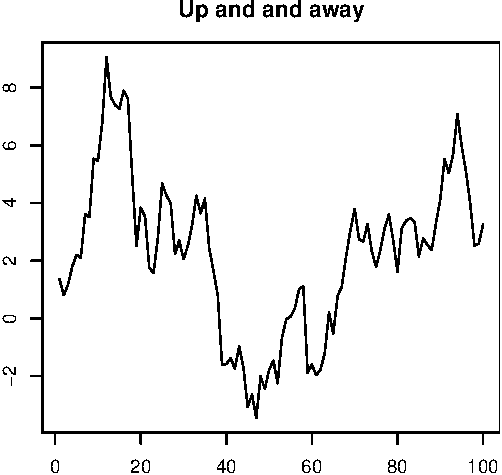
\includegraphics{pinp_files/figure-latex/unnamed-chunk-2-1} \end{center}

\hypertarget{pandoc}{%
\subsection{Pandoc}\label{pandoc}}

The easiest way to typeset code is to simply open three backticks
followed by the name of one of the \emph{numerous} built-in pandoc
parsers, \emph{i.e.}, \verb|```c| to typeset in the C languags.

\begin{Shaded}
\begin{Highlighting}[]
\CommentTok{/* this is a C function example */}
\DataTypeTok{int}\NormalTok{ doubleMe(}\DataTypeTok{int}\NormalTok{ x) \{}
    \ControlFlowTok{return}\NormalTok{ x + x;          }
\NormalTok{\}}
\end{Highlighting}
\end{Shaded}

Pandoc segments are highlighted as usual, and per a convention in this
template also shown in a framed and slightly shaded box as seen here and
above.

Another example from Python:

\begin{Shaded}
\begin{Highlighting}[]
\CommentTok{# A Python example}
\KeywordTok{def}\NormalTok{ printSomething(}\BuiltInTok{str}\NormalTok{):}
   \CommentTok{"This prints the string passed in"}
   \BuiltInTok{print} \BuiltInTok{str}
   
\end{Highlighting}
\end{Shaded}

\hypertarget{environments}{%
\section{Environments}\label{environments}}

\hypertarget{standard-latex}{%
\subsection{Standard LaTeX}\label{standard-latex}}

All standard LaTeX environment are directly usable if needed, including
of course all mathematical environments and symbols such as, say, the
greek lettering: \(\alpha\), \(\beta\), \(\gamma\), and so on.

The following is set as usual via the \texttt{displaymath} environment:

\begin{displaymath}
    a^2 = b^2 + c^2
\end{displaymath}

\hypertarget{figure}{%
\subsection{figure*}\label{figure}}

Figure can span two columns (when the default two-column mode is used)
by using a (LaTeX)
\texttt{\textbackslash{}begin\{figure*\}\ ...\ \textbackslash{}end\{figure*\textbackslash{}it\}}
environment, . Figures will then be \emph{floats} in the LaTeX sense and
place at the top or bottom of the page. An example is given by the
skeleton document of the package. Similarly,
\texttt{\textbackslash{}begin\{figure*\}\ ...\ \textbackslash{}end\{figure*\}}
could be used around a wide table structure.

\hypertarget{widetext}{%
\subsection{widetext}\label{widetext}}

The
\texttt{\textbackslash{}begin\{widetext\}\ ...\ \textbackslash{}end\{widetext\}}
environment can be used to break text from two-column mode to one-column
mode and back. As of the 2018 release of the underlying PNAS macros,
this feature is deprecated upstream. But both the \texttt{figure*} and
\texttt{table*} environments work, as does relying on \LaTeX commands
\texttt{\textbackslash{}onecolumn} and
\texttt{\textbackslash{}twocolumn}.

\hypertarget{other-help}{%
\section{Other Help}\label{other-help}}

\hypertarget{rmarkdown}{%
\subsection{RMarkdown}\label{rmarkdown}}

The \href{http://rmarkdown.rstudio.com/}{rmarkdown site} by RStudio is
very comprehensive and can answer many questions pertaining to Markdown
processing in R using the
\href{https://cran.r-project.org/package=rmarkdown}{rmarkdown package}.

\hypertarget{latex}{%
\subsection{LaTeX}\label{latex}}

Ultimately, this style uses LaTeX to produce the pdf output. The
\href{http://tex.stackexchange.com}{tex StackExchange} can be very
helpful for specific LaTeX questions.

%\showmatmethods
\showacknow




\begin{thebibliography}{3}
\newcommand{\enquote}[1]{``#1''}
\providecommand{\natexlab}[1]{#1}
\providecommand{\url}[1]{\texttt{#1}}
\providecommand{\urlprefix}{URL }
\expandafter\ifx\csname urlstyle\endcsname\relax
  \providecommand{\doi}[1]{doi:\discretionary{}{}{}#1}\else
  \providecommand{\doi}{doi:\discretionary{}{}{}\begingroup
  \urlstyle{rm}\Url}\fi
\providecommand{\eprint}[2][]{\url{#2}}

\bibitem[{Allaire \emph{et~al.}(2017)Allaire, {R Foundation}, Wickham, {Journal
  of Statistical Software}, Xie, Vaidyanathan, {Association for Computing
  Machinery}, Boettiger, {Elsevier}, Broman, Mueller, Quast, Pruim, Marwick,
  Wickham, Keyes, and Yu}]{CRAN:rticles}
Allaire J, {R Foundation}, Wickham H, {Journal of Statistical Software}, Xie Y,
  Vaidyanathan R, {Association for Computing Machinery}, Boettiger C,
  {Elsevier}, Broman K, Mueller K, Quast B, Pruim R, Marwick B, Wickham C,
  Keyes O, Yu M (2017).
\newblock \emph{rticles: Article Formats for R Markdown}.
\newblock R package version 0.4.1,
  \urlprefix\url{https://CRAN.R-project.org/package=rticles}.

\bibitem[{MacFarlane(2017)}]{pandoc}
MacFarlane J (2017).
\newblock \emph{Pandoc: A Universal Document Converter}.
\newblock Version 1.19.2.1, \urlprefix\url{http://pandoc.org}.

\bibitem[{Xie(2017)}]{CRAN:knitr}
Xie Y (2017).
\newblock \emph{knitr: A General-Purpose Package for Dynamic Report Generation
  in R}.
\newblock R package version 1.17, \urlprefix\url{https://yihui.name/knitr/}.

\end{thebibliography}

\end{document}

